\documentclass[11pt,a4paper]{article}

% ---------- Langue et encodage ----------
\usepackage[french]{babel}
\usepackage[utf8]{inputenc}
\usepackage[T1]{fontenc}
\usepackage{amssymb}

% ---------- Mise en page ----------
\usepackage[margin=2.5cm]{geometry}
\usepackage{graphicx}
\usepackage{xcolor}
\usepackage{booktabs}
\usepackage{array}
\usepackage{longtable}
\usepackage{enumitem}
\usepackage{fancyhdr}
\usepackage{titlesec}
\usepackage[colorlinks=true, linkcolor=blue!50!black, urlcolor=blue!50!black, citecolor=blue!50!black]{hyperref}
\usepackage{tcolorbox}
\tcbuselibrary{skins,breakable}
\usepackage{parskip}

% ---------- En-tete / pied de page ----------
\pagestyle{fancy}
\fancyhf{}
\fancyhead[L]{\small Cahier des charges --- Interop\'erabilit\'e en sant\'e}
\fancyhead[R]{\small Sujet B --- Rendez-vous / calendrier patient}
\fancyfoot[C]{\thepage}
\renewcommand{\headrulewidth}{0.4pt}

% ---------- Couleurs ----------
\definecolor{acompleterframe}{RGB}{200,120,0}
\definecolor{acompleterback}{RGB}{255,247,230}
\definecolor{diagframe}{RGB}{90,90,90}
\definecolor{diagback}{RGB}{245,245,245}

% ---------- Boite "a completer" ----------
\newtcolorbox{acompleter}[1][]{
  colback=acompleterback,
  colframe=acompleterframe,
  boxrule=1pt,
  arc=2pt,
  breakable,
  fonttitle=\bfseries,
  title={\`A COMPL\'ETER #1}
}

% ---------- Emplacement de diagramme ----------
\newtcolorbox{diagplaceholder}[2]{
  colback=diagback,
  colframe=diagframe,
  boxrule=0.75pt,
  arc=2pt,
  breakable,
  halign=center,
  valign=center,
  height=#2,
  fonttitle=\bfseries,
  title={#1}
}

\newcommand{\siu}{SIU\textasciicircum{}S12}

\title{\textbf{Cahier des charges}\\[0.3cm]
\large \'Evaluation --- Interop\'erabilit\'e en sant\'e\\
Sujet B --- Rendez-vous / calendrier patient}
\author{}
\date{}

\begin{document}

\begin{titlepage}
\centering
\vspace*{2cm}
{\Huge\bfseries Cahier des charges\par}
\vspace{0.5cm}
{\Large \'Evaluation --- Interop\'erabilit\'e en sant\'e\par}
\vspace{0.3cm}
{\large\itshape Sujet B --- Rendez-vous / calendrier patient\par}
\vspace{2cm}

\renewcommand{\arraystretch}{1.6}
\begin{tabular}{ll}
\textbf{Groupe} & Eya Rejeb, Neirouz Attia \\
\textbf{D\'ep\^ot GitHub} & \url{https://github.com/EyaRejeb/FHIR-interop} \\
\textbf{Sujet} & B --- Rendez-vous / calendrier patient \\
\textbf{Format cible} & HL7 v2 --- message \texttt{\siu} \\
\end{tabular}


\end{titlepage}

\tableofcontents
\newpage

% =====================================================================
\section{Besoin m\'etier, utilisateur, sc\'enario et crit\`eres d'acceptation}

\subsection{Utilisateur cible}
Le patient, via un portail num\'erique.

\subsection{Besoin m\'etier}
Permettre au patient de consulter la liste de ses rendez-vous \`a venir (extraits en temps r\'eel d'un serveur FHIR) et de prendre un nouveau rendez-vous, en garantissant que la donn\'ee cr\'e\'ee est imm\'ediatement interop\'erable avec le syst\`eme hospitalier cible via un message HL7 v2 SIU.

\subsection{Sc\'enario utilisateur (parcours)}
\begin{enumerate}[leftmargin=1.2cm]
  \item Le patient acc\`ede \`a son espace \og Mes rendez-vous \fg{} (identifiant patient saisi pour la d\'emo, pas d'authentification r\'eelle --- hors p\'erim\`etre du prototype).
  \item L'application interroge le serveur FHIR (\texttt{GET /Appointment?patient=...}) et affiche la liste des RDV \`a venir (date, praticien, motif, statut).
  \item Le patient choisit de prendre un nouveau RDV~: type de consultation, date/heure, praticien.
  \item L'application construit et envoie une ressource \texttt{Appointment} (\texttt{POST /Appointment}) au serveur FHIR.
  \item Une fois le RDV cr\'e\'e, l'application g\'en\`ere et affiche le message HL7 v2 \texttt{\siu} correspondant, tel qu'il serait transmis \`a un syst\`eme tiers (agenda du service, SI hospitalier).
  \item L'application affiche l'alignement terminologique effectu\'e (code FHIR source $\rightarrow$ code cible HL7 v2) pour au moins un champ cod\'e.
\end{enumerate}

\subsection{Crit\`eres d'acceptation}
\begin{itemize}[leftmargin=1.2cm]
  \item La liste des RDV affich\'ee provient r\'eellement du serveur FHIR (aucune donn\'ee m\'etier cod\'ee en dur).
  \item Un RDV cr\'e\'e via l'application est bien persist\'e c\^ot\'e serveur FHIR (v\'erifiable par une relecture \texttt{GET}).
  \item Le message HL7 v2 \texttt{\siu} g\'en\'er\'e est structurellement valide (segments MSH / SCH / PID / RGS--AIP--AIL coh\'erents).
  \item Le prototype g\`ere au moins un cas d'erreur (cr\'eneau invalide, serveur inaccessible, champ requis manquant) sans planter.
  \item Le mapping terminologique d'au moins un champ cod\'e (statut ou type de RDV) est visible et trac\'e dans l'interface.
\end{itemize}

% =====================================================================
\section{Choix des sp\'ecifications techniques}

\begin{table}[h!]
\centering
\renewcommand{\arraystretch}{1.5}
\begin{tabular}{p{3.2cm}p{4.2cm}p{6.5cm}}
\toprule
\textbf{\'El\'ement} & \textbf{Choix} & \textbf{Justification} \\
\midrule
Version FHIR & R4 & Version la plus largement support\'ee par les serveurs FHIR publics de test \\
Ressource principale & \texttt{Appointment} & Porte nativement \texttt{status}, \texttt{start}/\texttt{end}, \texttt{appointmentType}, \texttt{participant[]} \\
Ressources r\'ef\'erenc\'ees & \texttt{Patient}, \texttt{Practitioner}, \texttt{Location} & R\'ef\'erenc\'ees via \texttt{Appointment.\allowbreak participant[].\allowbreak actor} \\
Profil / IG & Base R4, sans profil sp\'ecifique par d\'efaut & \`A r\'eviser si le serveur retenu impose un IG \\
Standard cible & HL7 v2.x --- message \texttt{\siu} & Format explicitement impos\'e pour le Sujet B \\
Terminologies & \texttt{Appointment.status} (value set \texttt{appointmentstatus}) ; \texttt{Appointment.\allowbreak appointmentType} & Champs utilis\'es pour la vue \og changement de terminologie \fg \\
\bottomrule
\end{tabular}
\caption{Sp\'ecifications techniques retenues}
\end{table}

\begin{acompleter}[--- Serveur FHIR]
Indiquer ici l'URL de base du serveur FHIR utilis\'e, la version FHIR confirm\'ee via \texttt{GET~[base]/metadata} $\rightarrow$ \texttt{fhirVersion}, et si un profil/IG particulier est impos\'e par ce serveur. \\
\textbf{Point critique~:} confirmer que le \texttt{POST} (\'ecriture) est autoris\'e sur ce serveur avant de construire l'architecture de la Phase~2 dessus.
\end{acompleter}

\begin{acompleter}[--- Version HL7 v2 exacte]
Pr\'eciser la sous-version HL7 v2 retenue (2.3~/~2.4~/~2.5.1) --- les sous-champs des segments SCH, RGS, AIS, AIL, AIP peuvent l\'eg\`erement varier selon la version.
\end{acompleter}

% =====================================================================
\section{Interactions pr\'evues avec le serveur FHIR}

\begin{table}[h!]
\centering
\renewcommand{\arraystretch}{1.5}
\begin{tabular}{p{5.5cm}p{8.5cm}}
\toprule
\textbf{Appel} & \textbf{Usage} \\
\midrule
\texttt{GET /Appointment?patient=\{id\}\allowbreak\&date=ge\{today\}} & Recherche des RDV \`a venir du patient --- alimente la vue m\'etier \\
\texttt{GET /Appointment/\{id\}} & Lecture d\'etaill\'ee d'un RDV --- alimente la vue \og ressource FHIR brute \fg \\
\texttt{POST /Appointment} & Cr\'eation d'un nouveau RDV \\
\texttt{PUT /Appointment/\{id\}} \textit{(optionnel)} & Mise \`a jour de statut (ex. annulation) --- \`a ne traiter qu'apr\`es validation du \texttt{POST} \\
\bottomrule
\end{tabular}
\caption{Interactions FHIR pr\'evues}
\end{table}

% =====================================================================
\section{Architecture et lecture ReEIF}

\begin{longtable}{p{3.2cm}p{10.5cm}}
\toprule
\textbf{Couche ReEIF} & \textbf{Application au projet} \\
\midrule
\endhead
Infrastructure / s\'ecurit\'e & Acc\`es HTTPS au serveur FHIR ; pas d'authentification patient r\'eelle dans le prototype (identifiant saisi librement pour la d\'emo) --- limite assum\'ee, \`a mentionner explicitement \`a l'oral \\
Application & L'application web est un client FHIR (appels REST) ; le serveur FHIR fait office de backend unique, aucune base de donn\'ees locale propre au prototype \\
Information & Structure de la ressource \texttt{Appointment} (dates, participants, statut, type) et son \'equivalent en segments SIU (SCH, AIP, AIL, PID) \\
M\'etier & Processus de prise de RDV c\^ot\'e patient~: qui peut cr\'eer un RDV, quelles r\`egles sont r\'eellement v\'erifi\'ees (ex. cr\'eneau non vide) vs simplifi\'ees pour la d\'emo \\
Organisation & Dans un contexte r\'eel, le message SIU serait re\c{c}u par l'agenda du service ou le secr\'etariat ; dans le prototype, ce destinataire est simul\'e \\
Juridique & Consentement du patient et RGPD sur les donn\'ees de rendez-vous (cat\'egorie de donn\'ee de sant\'e sensible m\^eme si le contenu est peu clinique) --- \`a mentionner comme limite du prototype \\
\bottomrule
\caption{Lecture ReEIF du projet}
\end{longtable}

% =====================================================================
\section{R\`egles de transformation et de mapping s\'emantique}

\begin{table}[h!]
\centering
\renewcommand{\arraystretch}{1.5}
\begin{tabular}{p{5.5cm}p{7.5cm}}
\toprule
\textbf{Champ FHIR \texttt{Appointment}} & \textbf{\'El\'ement HL7 v2 \texttt{\siu}} \\
\midrule
\texttt{status} & Statut du filler port\'e par le segment SCH \\
\texttt{start} / \texttt{end} & Cr\'eneau horaire du rendez-vous, port\'e par SCH \\
\texttt{appointmentType} & Table de codes cible (v2-0276 ou table locale document\'ee) \\
\texttt{participant[Patient]} & Segment PID \\
\texttt{participant[Practitioner]} & Segment AIP (Personnel Resource), sous un groupe RGS \\
\texttt{participant[Location]} & Segment AIL (Location Resource), sous un groupe RGS \\
\bottomrule
\end{tabular}
\caption{Mapping FHIR \texorpdfstring{$\rightarrow$}{->} HL7 v2 SIU}
\end{table}

\subsection*{Limites et pertes d'information identifi\'ees}
\begin{itemize}[leftmargin=1.2cm]
  \item FHIR autorise un statut individuel par participant (\texttt{Appointment.\allowbreak participant[].\allowbreak status})~; SIU repr\'esente cette information de fa\c{c}on plus rigide via des segments r\'ep\'et\'es (RGS/AIP/AIL), sans porter aussi finement un statut par ressource --- perte de granularit\'e potentielle.
  \item Certains champs FHIR sans \'equivalent direct dans SIU (ex.\ \texttt{Appointment.\allowbreak comment}, \texttt{Appointment.\allowbreak basedOn}) seront soit omis, soit report\'es en note libre (segment NTE) --- perte d'information structur\'ee.
  \item Toute correspondance de code (\texttt{appointmentType} notamment) qui n'a pas d'\'equivalent exact dans la table cible sera document\'ee comme approximation assum\'ee, pas comme un mapping garanti sans perte.
\end{itemize}

% =====================================================================
\section{Vues attendues pour la Phase 2 (r\'ealisation)}

\begin{enumerate}[leftmargin=1.2cm]
  \item \textbf{Vue m\'etier}~: liste des RDV du patient + formulaire de prise de RDV.
  \item \textbf{Vue ressource FHIR}~: affichage brut (JSON) de la ou des ressources \texttt{Appointment} r\'eellement utilis\'ees.
  \item \textbf{Vue conversion}~: affichage du message HL7 v2 \texttt{\siu} g\'en\'er\'e \`a partir de la ressource FHIR.
  \item \textbf{Vue mapping terminologique}~: tableau ou affichage code source (FHIR) $\rightarrow$ code cible (HL7 v2) pour le statut et/ou le type de RDV.
  \item \textbf{Gestion d'erreurs et tra\c{c}abilit\'e}~: messages d'erreur explicites en cas d'\'echec d'appel FHIR, journal minimal des \'echanges (requ\^ete/r\'eponse) affich\'e ou logg\'e.
\end{enumerate}

% =====================================================================
\section{Diagrammes}

\subsection{Diagramme BPMN du processus}
Diagramme du parcours complet en notation BPMN standard (pool + 4 couloirs~: Patient, Application, Serveur FHIR, Syst\`eme tiers), de la consultation des RDV jusqu'\`a la g\'en\'eration du message HL7~v2, y compris le chemin d'erreur.

\begin{figure}[h!]
\centering
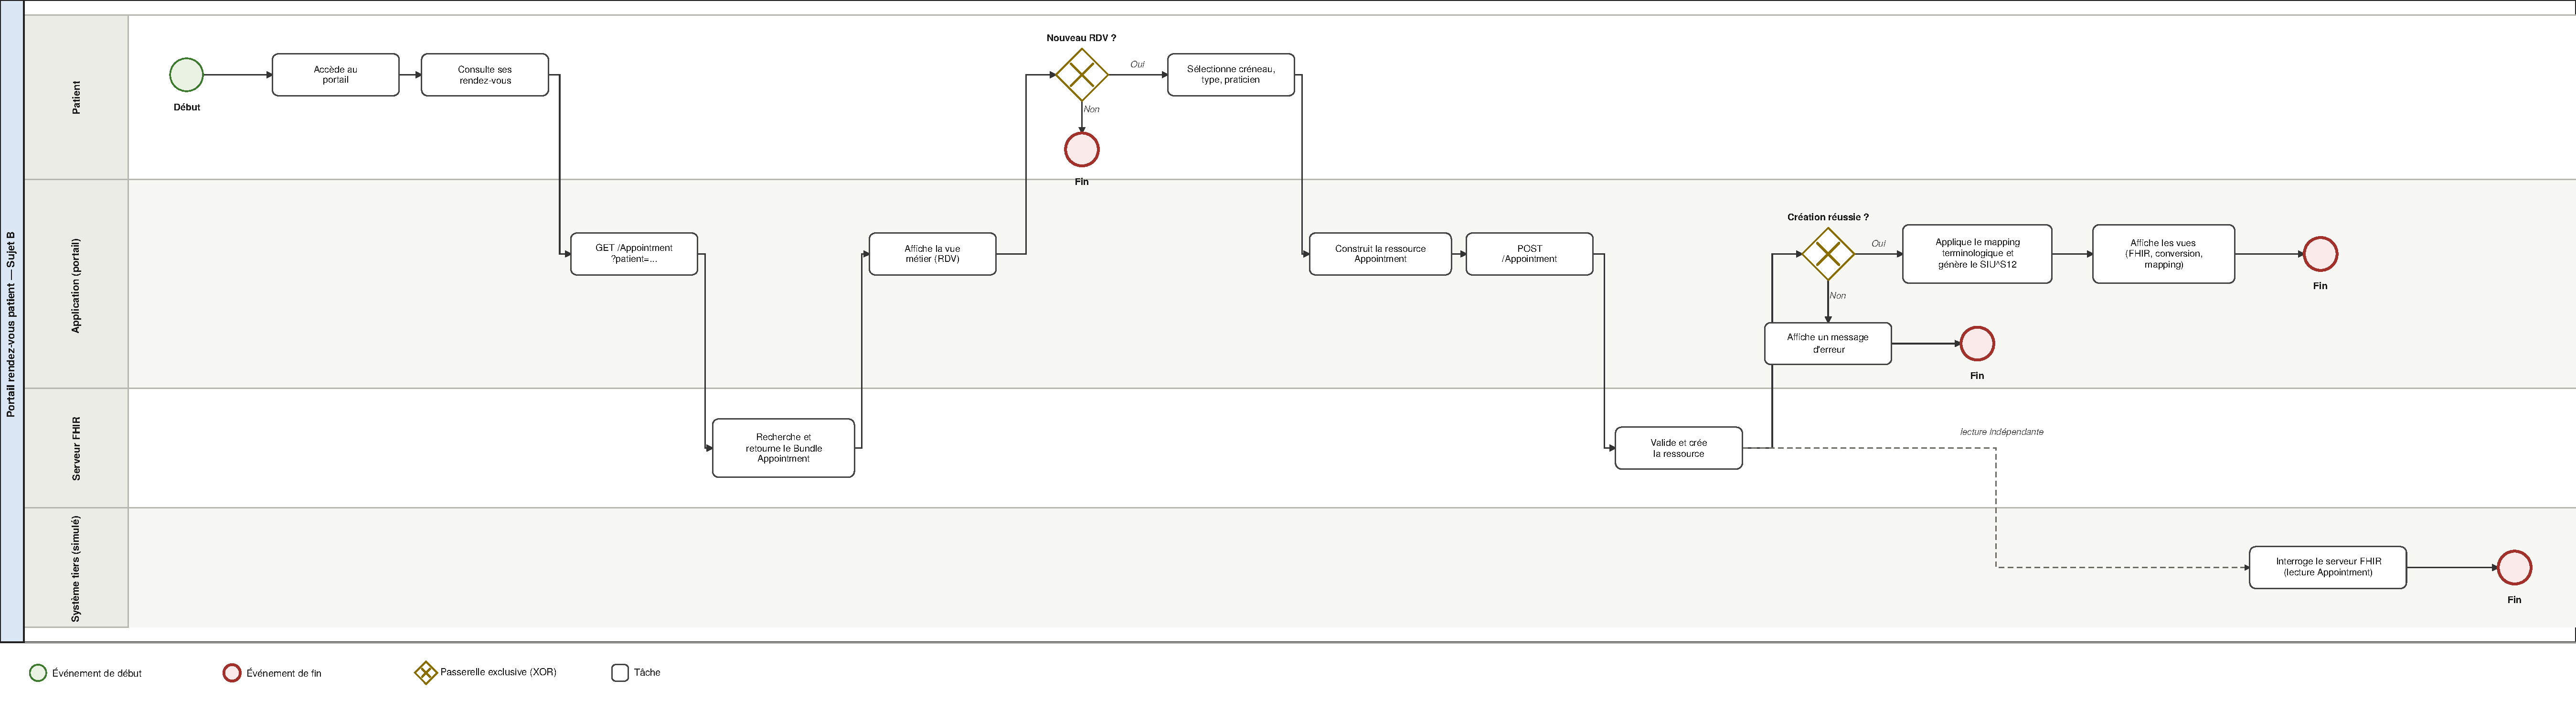
\includegraphics[width=0.95\textwidth]{figures/bpmn-sujetb.pdf}
\caption{Diagramme BPMN du parcours --- Sujet B}
\label{fig:bpmn}
\end{figure}

\newpage
\subsection{Diagramme de cas d'utilisation}
Repr\'esente les acteurs (Patient, \'eventuellement Syst\`eme tiers) et les cas d'utilisation principaux~: consulter ses RDV, cr\'eer un RDV, visualiser la conversion HL7~v2, visualiser le mapping terminologique.

\begin{figure}[h!]
\centering
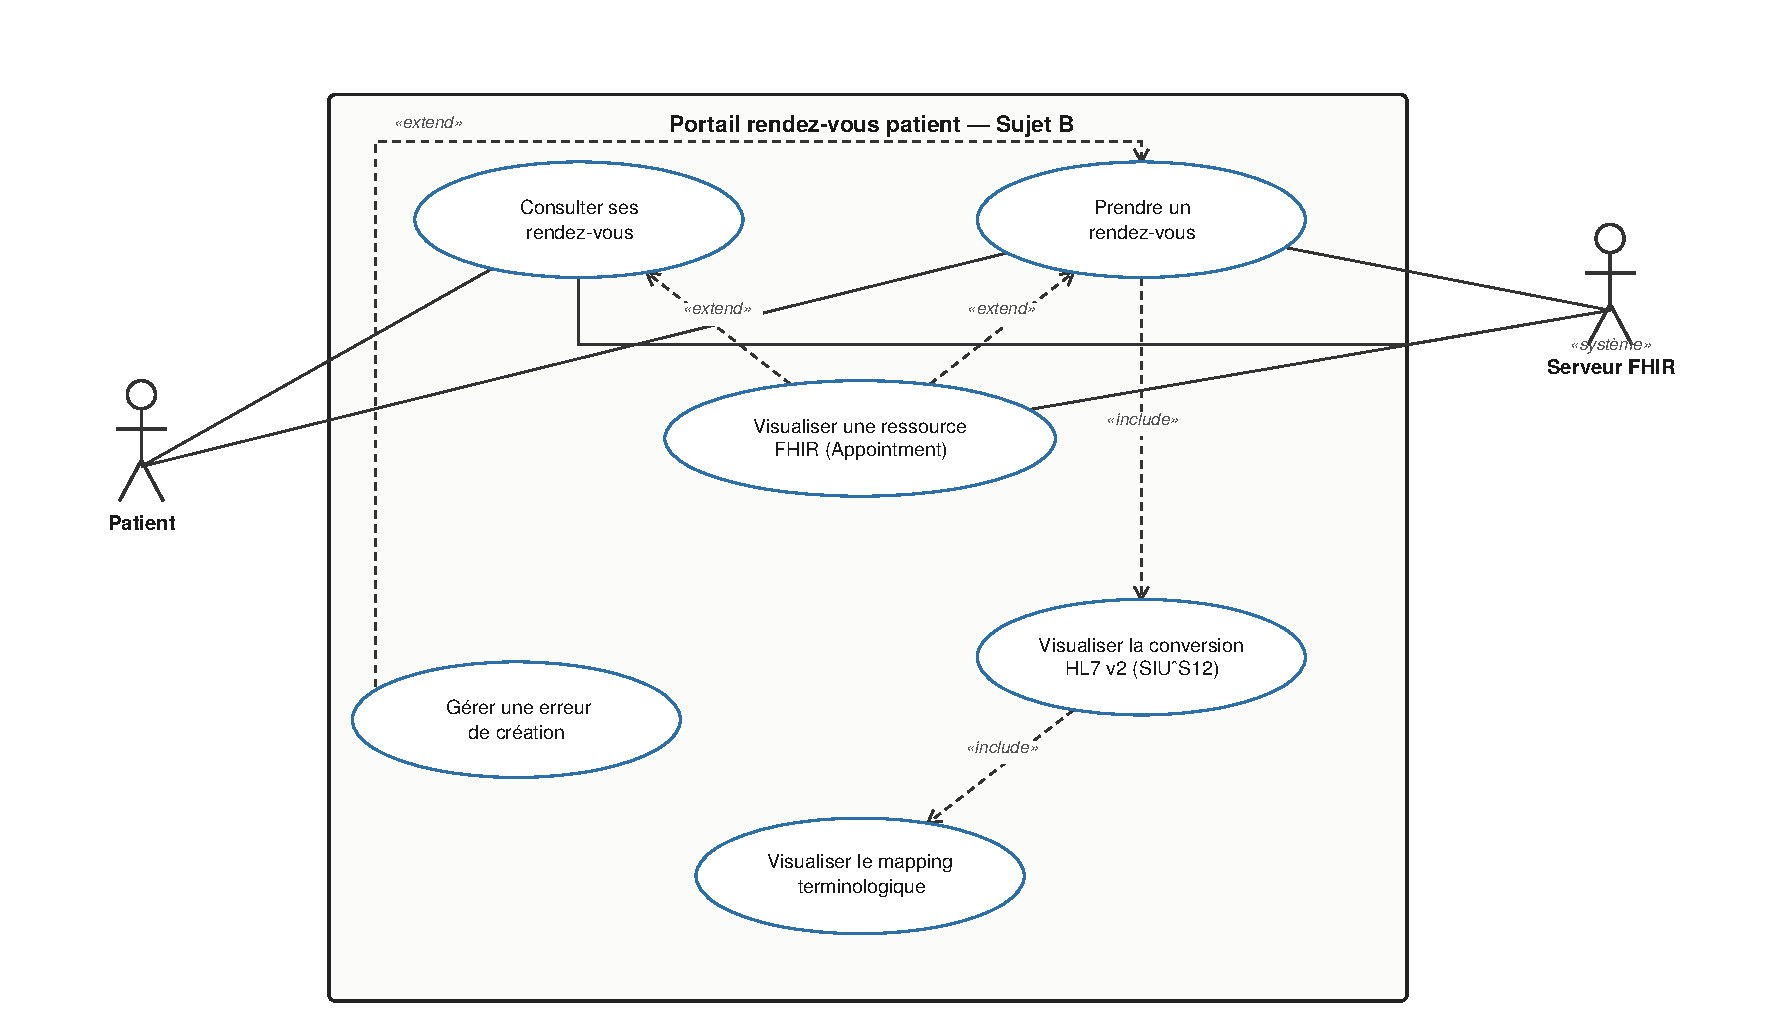
\includegraphics[width=0.95\textwidth]{figures/cas-utilisation.pdf}
\caption{Diagramme de cas d'utilisation --- Sujet B}
\label{fig:usecase}
\end{figure}

\newpage
\subsection{Diagramme de s\'equence}
D\'etaille les \'echanges temporels entre le Patient, l'Application, le Serveur FHIR et le Syst\`eme tiers (simul\'e), pour le sc\'enario de cr\'eation de RDV avec conversion HL7~v2.

\begin{figure}[h!]
\centering
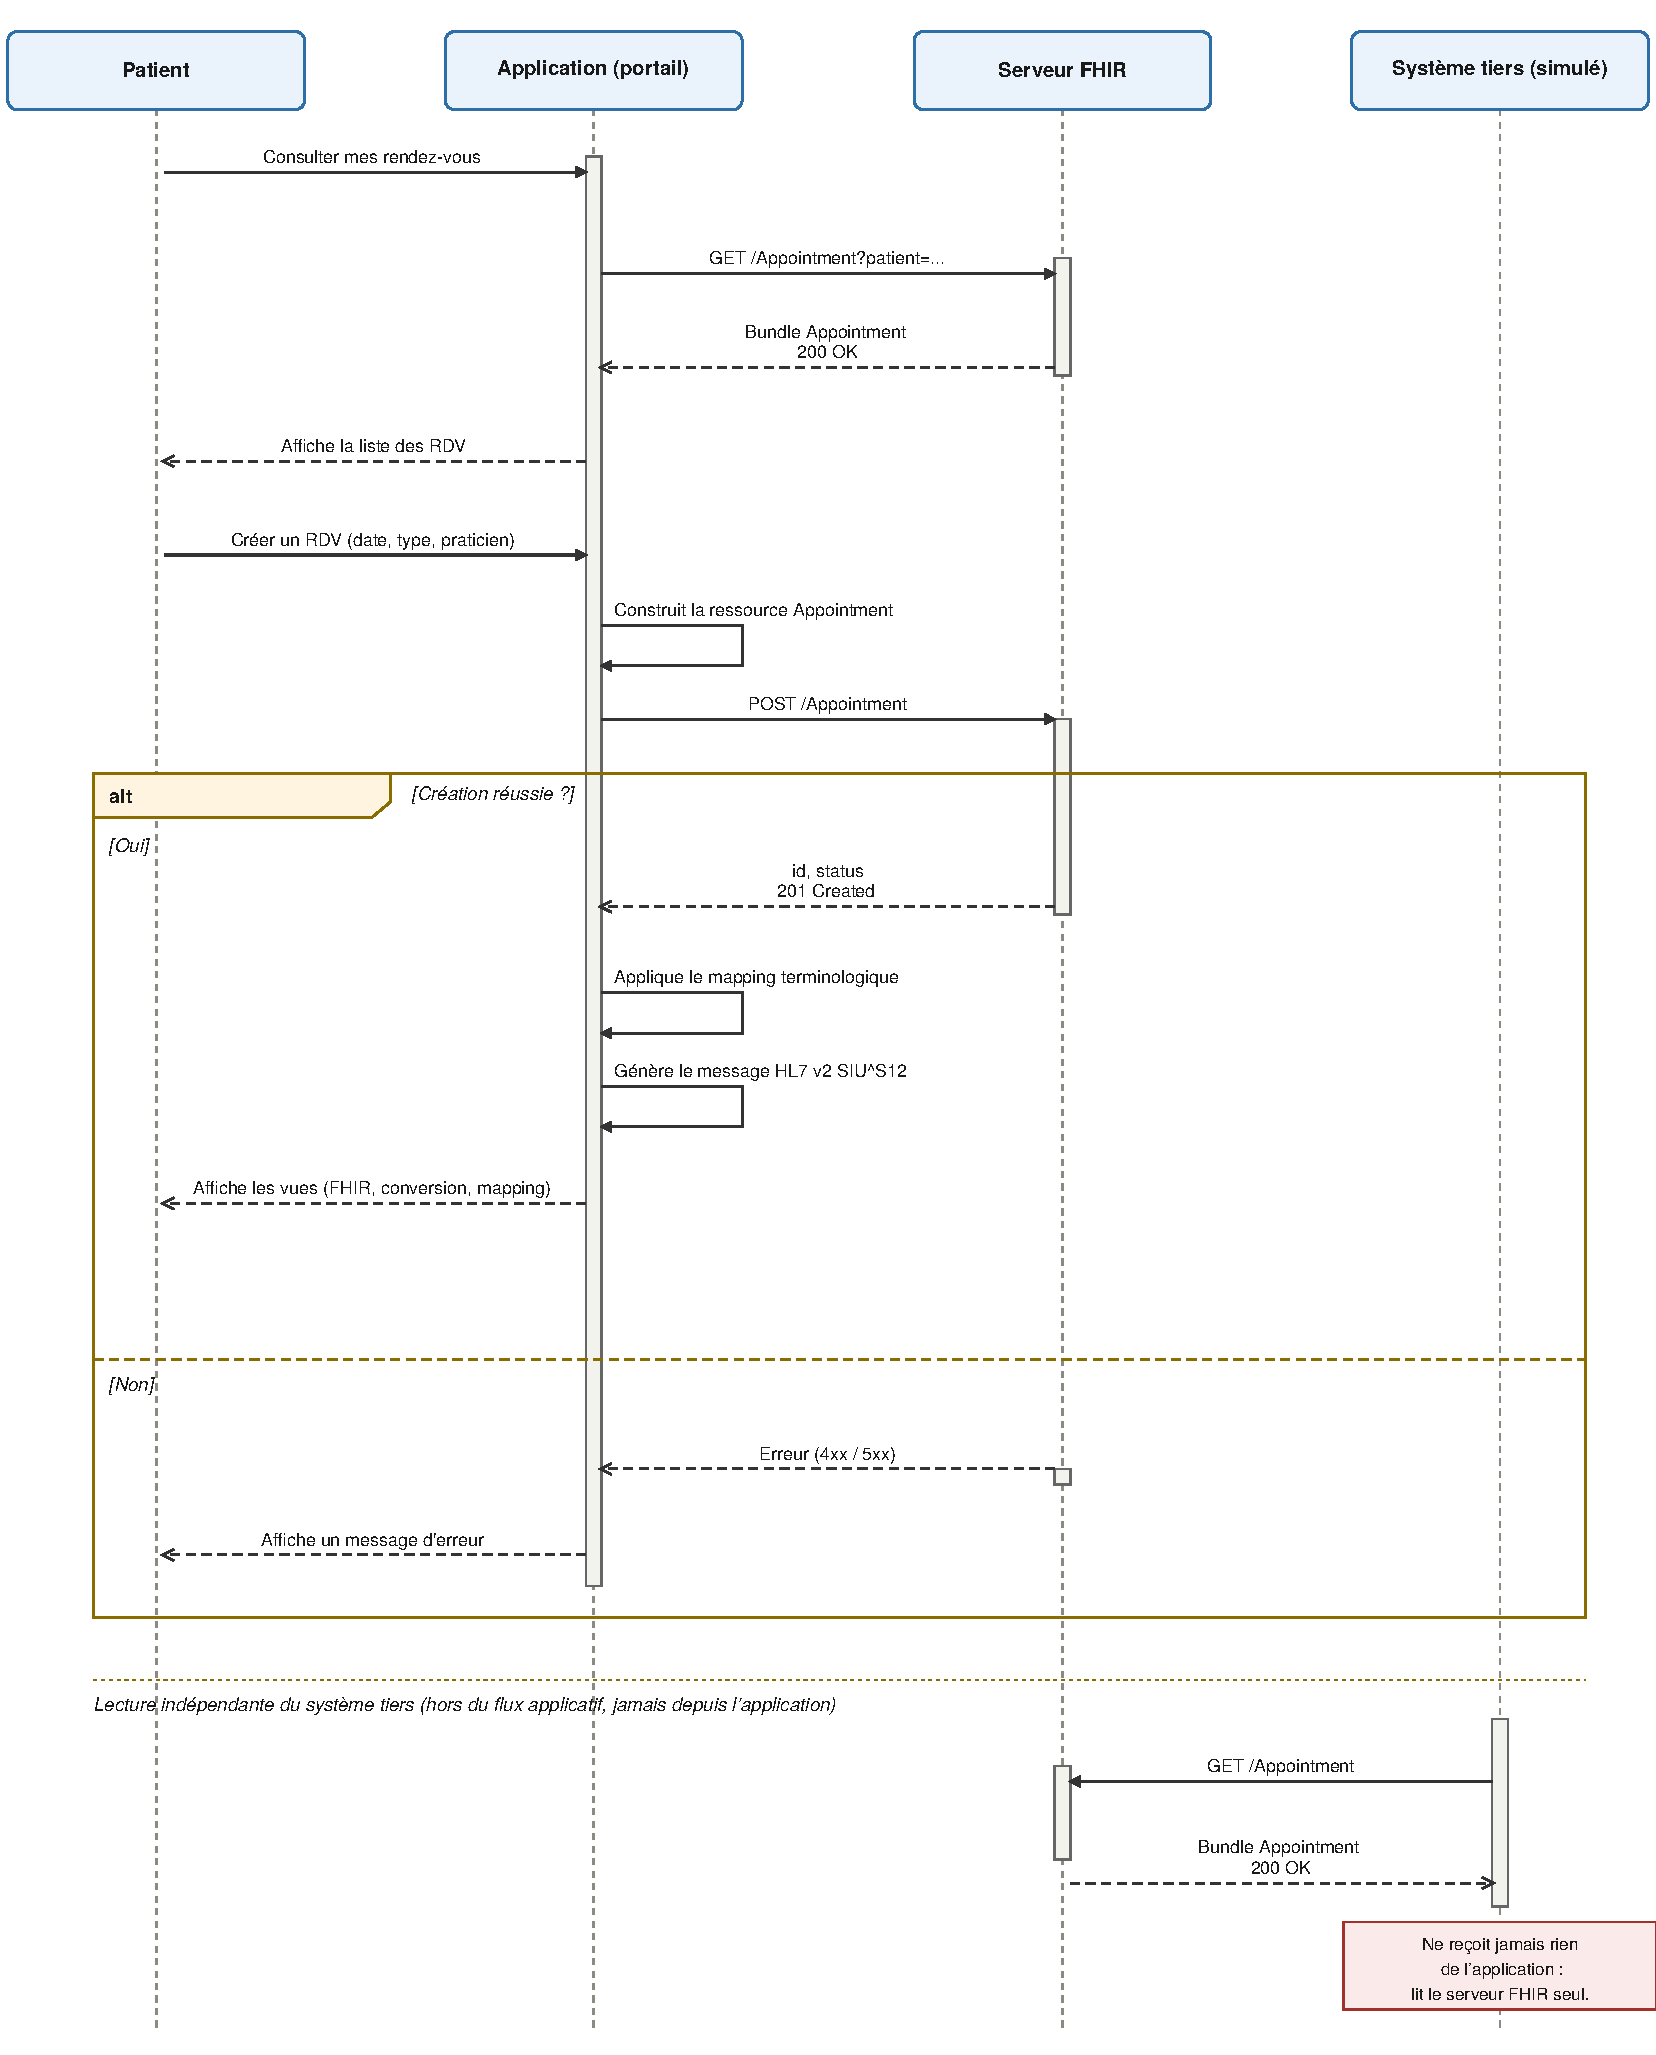
\includegraphics[width=0.95\textwidth]{figures/sequence.pdf}
\caption{Diagramme de s\'equence --- cr\'eation d'un RDV}
\label{fig:sequence}
\end{figure}

\newpage
\subsection{Diagramme de d\'eploiement}
Repr\'esente les n\oe uds physiques/logiques~: poste client (navigateur), application (portail), serveur FHIR, et le syst\`eme tiers simul\'e, avec les protocoles d'\'echange (HTTPS/REST).

\begin{figure}[h!]
\centering
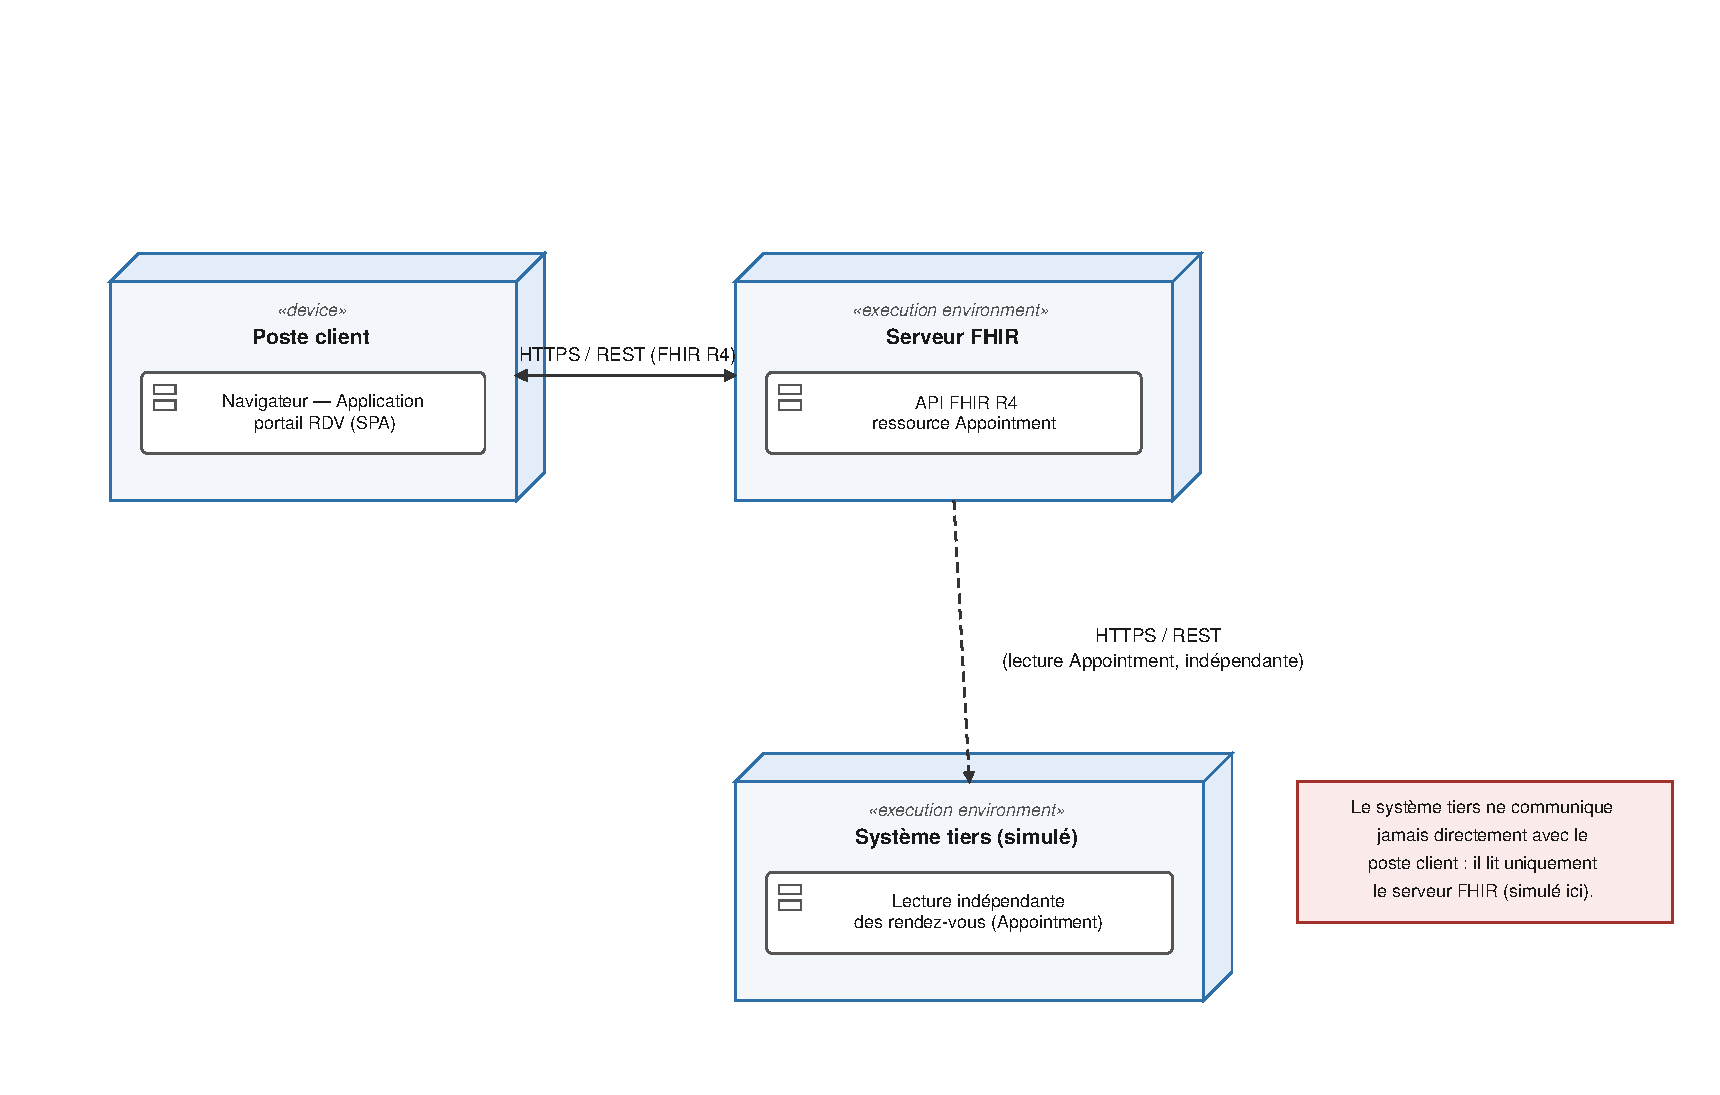
\includegraphics[width=0.95\textwidth]{figures/deploiement.pdf}
\caption{Diagramme de d\'eploiement --- Sujet B}
\label{fig:deployment}
\end{figure}

\begin{acompleter}[--- Diagramme de d\'eploiement]
Pr\'eciser si l'application est h\'eberg\'ee localement ou sur un service cloud pour la d\'emonstration, et confirmer l'URL r\'eelle du serveur FHIR utilis\'e (cf.\ encadr\'e section~2).
\end{acompleter}

% =====================================================================
\section{Points \`a v\'erifier avant la Phase 2}

\begin{itemize}[leftmargin=1.2cm]
  \item[$\square$] Confirmer l'URL du serveur FHIR utilis\'e et sa version (\texttt{GET~[base]/metadata}).
  \item[$\square$] \textbf{Tester que le \texttt{POST /Appointment} fonctionne r\'eellement} sur ce serveur avant de construire toute l'architecture dessus (risque majeur~: certains serveurs FHIR publics sont en lecture seule ou r\'einitialis\'es r\'eguli\`erement).
  \item[$\square$] V\'erifier si le serveur impose un profil/IG particulier sur \texttt{Appointment}.
  \item[$\square$] Valider la structure exacte du message \texttt{\siu} par rapport \`a la version HL7~v2.x retenue.
\end{itemize}

\begin{acompleter}[--- \'Etat des v\'erifications]
Une fois les points ci-dessus contr\^ol\'es, cocher chaque case et noter ici les r\'esultats (ex.\ URL confirm\'ee, r\'esultat du test \texttt{POST}, version HL7 retenue) avant de transmettre ce document \`a l'IA de d\'eveloppement pour la Phase~2.
\end{acompleter}

\end{document}
